\documentclass{book}
\usepackage{lmodern}
\usepackage{amsmath}
\usepackage{amssymb}
\usepackage{amsfonts}
\usepackage{xcolor}
\usepackage{mdframed}
\usepackage[top=3cm, bottom=3cm, inner=4cm, outer=3cm]{geometry}
\usepackage{hhline}
\usepackage{graphicx}

\DeclareMathOperator{\lcm}{lcm}
\DeclareMathOperator{\bigo}{\mathcal{O}}

\newenvironment{task}
  {\begin{mdframed}[backgroundcolor=lightgray]}
  {\end{mdframed}}
  
\begin{document}

\chapter{Solutions}

\section{Multiples of 3 and 5}

\begin{task}
If we list all the natural numbers below $10$ that are multiples of $3$ and $5$, we get $3$, $5$, $6$, and $9$. The sum of these multiples is $23$.\\
\\
Find the sum of all the multiples of $3$ and $5$ below $1000$.
\end{task}

The first problem is pretty much straightforward. It asks us to find the sum of all multiples of $3$
and $5$, but any multiple must not exceed $1000 - 1 = 999$. But wait, is this task really that simple?
The only trick is that when we calculate the multiples, some of the multiples of $3$ and $5$ are the
same, e.g. $15$, $30$, ... That means, that if we do not implement this task in smart way, some of the
multiples might get counted twice. Those numbers are exactly the multiples of the least common
multiple of $3$ and $5$, which is $15$. We denote that as $\lcm(3, 5) = 15$.\\

Let us take a look at naive solution:

\begin{verbatim}
#include<stdio.h>

int main()
{
    int sum = 0;
    for (int i = 1; i <= 333; i++)   // we iterate from 1 to (int)999/3 = 333
        sum += 3 * i;
    for (int i = 1; i <= 199; i++)   // we iterate from 1 to (int)999/5 = 199
        sum += 5 * i;
    for (int i = 1; i <= 66; i++)    // we iterate from 1 to (int)999/15 = 66
        sum -= 15 * i;               // we must subtract the twice counted numbers
    printf("%d\n", sum);

    return 0;
}
\end{verbatim}

Note that if you implement this program, it will print the value instantly, therefore you might pose the question, why is this a naive solution?
The reasons are two. Firstly, we use three for loops. That results in asymptotic complexity of $\bigo(m/x + m/y + m/ \lcm(x, y))$, where $x$ and $y$ are the numbers whose multipliers we want to sum and $m$ is the upper bound for all multiples. Now consider we are given extremely large numbers. Although the program runs in linear time, it will take more and more time to get through those three loops. We can clearly see, that we could get rid of three loops and make only one loop, as in next implementation. Wait until you see the real reason why this implementation is not as beautiful as it could be (not to mention it is tiresomly slow - oh, wait, linear is slow, can you do it faster, let’s say logarithmic? Hell no, CONSTANT!).

\begin{verbatim}
#include<stdio.h>

int main()
{
    int sum = 0;
    for (int i = 3; i < 1000; i++)
    {
        if (i % 3 == 0 || i % 5 == 0)
            sum += i;
    }
    printf("%d\n", sum);
    
    return 0;
}
\end{verbatim}

Note that this implementation does not require any subtraction of multiples of $15$, because we check every integer between $3$ and $999$ inclusively only once. We also expect this program to run slower then the three for one, because in this case we have to loop through $m - 2 = 998$ numbers and each time check whether that number is a multiple of $3$ or $5$, whereas in three for loop we only loop through $\lfloor(m - 1)/x\rfloor + \lfloor(m - 1)/y\rfloor + \lfloor(m - 1)/ \lcm(x, y)\rfloor = 333 + 199 + 66 = 598$ numbers and we do not need to do any checks.

The second reason, and here starts the real solution to the problem, is that what we are doing is actually computing a sum of three \textit{arithmetic series}. An arithmetic series is a sum of numbers that are computed using relation \[a_1;~~~a_i = a_1 + d(i-1),\] where $d$ denotes a difference or \textit{distance} between two numbers in series. In our case we have three arithmetic series, first given by \[a_1 = 3;~~a_i = 3 + 3(i-1) = 3i,\] the second by \[b_1 = 5;~~b_i = 5 + 5(i-1) = 5i\] and the third by \[c_1 = 15;~~c_i = 15 + 15(i-1) = 15i.\] We are actually subtracting the sum of $\{c_i\}_{i = 1}^{66}$ series.
Now, beautiful mathematics gives us a formula for computing sum of arithmetic series. The formula is \[\sum_{i=1}^n a_i = \frac{n}{2}(a_1 + a_n).\] Since in our case $a_n = 3n$, $b_n = 5n$, and $c_n = 15n$, the above equation simplifies into \[\sum_{i=1}^n a_i = a_1 \cdot \frac{n(n+1)}{2}.\] You can simply make your own calculations to see that formula is indeed correct. Let us now implement the program WITHOUT any \texttt{for} loops at all! We use a formula derived above and get \[\textrm{sum} = \sum_{i=1}^{333} 3i + \sum_{i=1}^{199} 5i - \sum_{i=1}^{66} 15i = 3\cdot\frac{333\cdot334}{2} + 5\cdot\frac{199\cdot200}{2} - 15\cdot\frac{66\cdot67}{2}.\]

\begin{verbatim}
#include<stdio.h>
#include "campovski.h"               // needed for GCD function

int main()
{
    int x, y, m;                     // we let user input starting numbers
    scanf("%d %d %d, &x, &y, &m);    // (in our case "3 5 1000")
    m--;                             // number below m, m not included (1000-1)
    
    int z = x * y / gcd(x, y);       // LCM(x,y) = x * y / GCD(x,y)
    int n1 = (int) m / x;            // calculate range of sum for x (3)
    int n2 = (int) m / y;            // calculate range of sum for y (5)
    int n3 = (int) m / z;            // calculate range of sum for LCM(x,y) (15)
    
    int sum = x * n1 * (n1 + 1) / 2;
    sum += y * n2 * (n2 + 1) / 2;
    sum -= z * n3 * (n3 + 1) / 2;
    
    printf("%d\n", sum);
    
    return 0; 
}
\end{verbatim}

You might say taht you could do that faster with your own calculator. Well, the beauty of coding is finding mathematical background of given problem and optimizing the solution.\\

I tested all three of the above programs with number $x = 3$, $y = 5$, and $m \in \{10^3, 10^6, 10^9, 10^{12}\}$. The results are astounding (see table below). I also had to change \texttt{int}s to \texttt{long long}s.

\begin{table}[h!]
\centering
\begin{tabular}{||l||c|c|c|c||}
\hhline{|t:=====:t|}
\textit{Algorithm} & $t(m = 10^3)$ & $t(m = 10^6)$ & $t(m=10^9)$ & $t(m=10^{12})$\\
\hhline{||=||=|=|=|=||}
Three \texttt{for} loops & $0.000002$ & $0.001528$ & $1.384336$ & $1321.064965$\\
\hline
One \texttt{for} loop & $0.000004$ & $0.003579$ & $3.020462$ & \\
\hline
Formula & $< 0.000001$ & $< 0.000001$ & $< 0.000001$ & $< 0.000001$\\
\hhline{|b:=====:b|}
\end{tabular}
\caption{Table shows running time (in seconds) of given algorithms in relation to $m$. Time was measured with help of \texttt{time.h}.}
\end{table}

Note, hot lovely are the running times of first two algorithms increasing with $m$. Thousand times greater problem, thousand times more time needed. The third algorithm obviously runs in constant time.

\pagebreak

%%%%%%%%%%%%%%%%%%%%%%%%%%%%%%%%%%%%%%%%%%%%%%%%%%%%%%%%%%%%%%%%%%%%%%%%%%%%%%%%%%%%%%%%%%%%%%%%%%%%%%
%%%%%%%%%%%%%%%%%%%%%%%%%%%%%%%%%%%%%%%%%%%%%%%%%%%%%%%%%%%%%%%%%%%%%%%%%%%%%%%%%%%%%%%%%%%%%%%%%%%%%%
%%%%%%%%%%%%%%%%%%%%%%%%%%%%%%%%%%%%%%%%%%%%%%%%%%%%%%%%%%%%%%%%%%%%%%%%%%%%%%%%%%%%%%%%%%%%%%%%%%%%%%
%%%%%%%%%%%%%%%%%%%%%%%%%%%%%%%%%%%%%%%%%%%%%%%%%%%%%%%%%%%%%%%%%%%%%%%%%%%%%%%%%%%%%%%%%%%%%%%%%%%%%%

\section{Even Fibonacci numbers}

\begin{task}
Each new term in the Fibonacci sequence is generated by adding the previous two terms. By starting with $1$ and $2$, the first $10$ terms will be: \[1,2,3,5,8,13,21,34,55,89,\dotsc\]

By considering the terms in the Fibonacci sequence whose values do not exceed four million, find the sum of the even-valued terms.
\end{task}

Let us start with example from the task. The first ten terms of Fibonacci sequence, as the task states it, are $1$, $2$, $3$, $5$, $8$, $13$, $21$, $34$, $55$, and $89$. Even-valued terms, that do not exceed $34$ are $2$, $8$, and $34$. Therefore, the sum of the even-valued terms that do not exceed $34$ is $2+8+34 = 44$.\\

Before we get into programming, let us first discuss how terms of Fibonacci sequence are calculated. The first two terms, according to task, are $F_1 = 1$ and $F_2 = 2$. (Mind, that some sources state Fibonacci sequence as $1$, $1$, $2$, $3$, $5$, $8$, $13$,... or even $0$, $1$, $1$, $2$, $3$, $5$, $8$, $13$,...) The next term is acquired by adding previous two together. We end up with formula \[F_n = F_{n-1} + F_{n-2};~n \geq 3.\] This is recursive formula with starting values of $F_1 = 1$ and $F_2 = 2$. At this point you might think that we are going to recursion in order to calculate terms of Fibonacci sequence, but we are not. The reason is, that if we want to compute $n$-th term of Fibonacci sequence, we can use recursion. In our case, we do not know what term is the first that exceeds $4000000$, therefore we cannot use recursion. Besides, naive recursion (if we could use it) would calculate the same terms over and over again - see figure below. We could use a concept called \textit{memoization} and get rid of this problem, but as I said, we cannot use this technique in this situation.

\begin{figure}[h!]
\centering
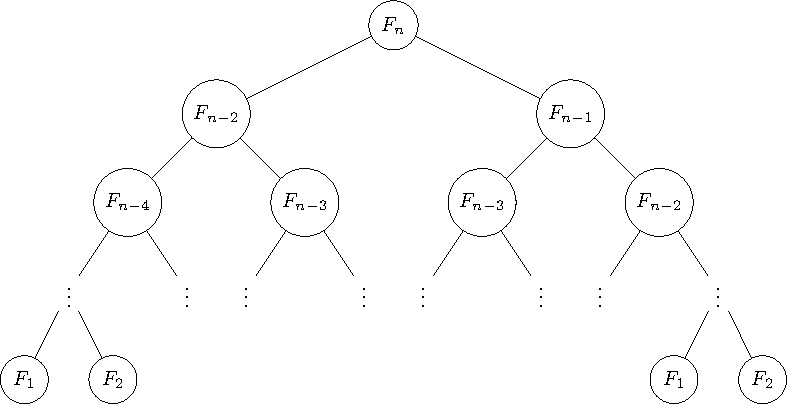
\includegraphics[scale=1]{images/002-tree.pdf}
\caption{Recursion tree for Fibonacci sequence. Note, how terms keep repeating.}
\end{figure}

Since we cannot use recursion from $n$ to $1$, we are going to go from $1$ to $n$, summing the previous two terms together to obtain the next one. We are going to check whether that term is even and if it is, we are going to add it to sum.

\begin{verbatim}
#include<stdio.h>

int main()
{
    int x = 1;             // x represents F(n-2)
    int y = 2;             // y represents F(n-1)
    int tmp;               // tmp represents F(n)
    int sum = 0;
    while (x <= 4000000)
    {
        if (!(x % 2))      // check if x is even
            sum += x;
        tmp = x + y;       // F(n) = F(n-1) + F(n-2)
        x = y;             // F(n-1) becomes F(n-2) for next iteration
        y = tmp;           // F(n) becomes F(n-1) for next iteration
    }
    printf("%d\n", sum);
    
    return 0;
}
\end{verbatim}

There are probably few things I should explain. First is the condition in \texttt{if} clause. In C, as well as in some other languages, number $0$ of type \texttt{int}, beside of being a regular number, stands for $\textit{false}$ (mind, that C does NOT have boolean variables). Thus, we do not need to make comparison of \texttt{0 == 0}, but we can simply write \texttt{!0}, which evaluates to \texttt{1}.
Next thing is the way we compute terms for next iteration. First, we sum current terms and save the result in temporary variable \texttt{tmp}. Then we rewrite \texttt{x} and \texttt{y} with \texttt{y} and \texttt{tmp} respectively, thus shifting the sequence to the left. The asymptotic complexity of this algorithm is $\bigo(n)$, where $n$ is the number which terms must not exceed - in our case $n = 4000000$.\\

Remember, that I said that some sources state Fibonacci sequence as $1$, $1$, $2$, $3$, $5$, $8$, $13$, $21$, $44$,... Observing this sequence for long enough we can see, that even-valued terms are $F_{3i}$ for all $i \in \mathbb{N}$. Proving this is simple. The sum of two odd numbers is even and the sum of even and odd number is odd. Looking at the sequence we can see that this proves the statement by law of induction. Therefore, we can be sure that if we add every third term of Fibonacci sequence to our final sum, we will obtain the correct result. The following algorithm does exactly that. Each iteration we compute the next three terms of Fibonacci sequence and always add the third to final sum.

\begin{verbatim}
#include<stdio.h>

int main()
{
    int x = 1;             // x represents F(n-2) - always odd
    int y = 1;             // y represents F(n-1) - always odd
    int z = 2;             // z represents F(n) - the even term
    int sum = 0;
    
    while (z <= 4000000)
    {
        sum += z;          // always add z since it is always even
        x = y + z;         // F(n+1) = F(n-1) + F(n) (x becomes F(n-2))
        y = z + x;         // F(n+2) = F(n) + F(n+1) (y becomes F(n-1))
        z = x + y;         // F(n+3) = F(n+2) + F(n+2) (z becomes F(n))
    }
    
    printf("%d\n", sum);
    
    return 0;
}
\end{verbatim}

This algorithm still runs in $\bigo(n)$ but we are advancing three times faster than in previous algorithm, because we calculate three terms in each iteration of \texttt{while} loop and omitting the \texttt{if} clause, thus expecting this algorithm to run approximately three times faster does not sound stupid. The only problem is that we are also doing more summations, which will result in algorithm not being three times as fast as the previous one, but it should still be faster.\\

Now it is time for some maths. We already figured out that even-valued terms are $F_{3i}$. If we manage to rewrite the recusrion formula $F_n = F_{n-1} + F_{n-2}$ into $F_n = \alpha f_{n-3} + \beta F_{n-6}$, we will obtain a formula that uses only every third Fibonacci number and we will not have to bother with odd-valued terms. Let us try to do that.
\begin{align*}
F_n &= F_{n-1} + F_{n-2}\\
&= (F_{n-2} + F_{n-3}) + (F_{n-3} + F_{n-4})\\
&= \big((F_{n-3} + F_{n-4}) + F_{n-3}\big) + \big(F_{n-3} + (F_{n-5} + F_{n-6})\big)\\
&= 3F_{n-3} + (F_{n-4} + F_{n-5}) + F_{n-6}\\
&= 4F_{n-3} + F_{n-6}
\end{align*}
Easy peasy lemon squizy! Based on formula derived, we can implement next program.

\begin{verbatim}
#include<stdio.h>

int main()
{
    int x = 2;             // x represents F(n-6)
    int y = 8;             // y represents F(n-3)
    int tmp;               // tmp represents F(n)
    int sum = 0;
    
    while (x <= 4000000)
    {
        sum += x;
        tmp = 4 * y + x;   // F(n) = 4 * F(n-3) + F(n-6)
        x = y;             // F(n-3) becomes F(n-6) for next iteration
        y = tmp;           // F(n) becomes F(n-3) for next iteration
    }
    
    printf("%d\n", sum);
    
    return 0;
}
\end{verbatim}

Can you guess, how much faster, if faster, will this algorithm run compared to the second one? It still runs in $\bigo(n)$, we still advance by three terms each iteration... But hey, did you forget about the number of operations again?! I hope not. This time, we do one multiplication more than in second algorithm, but two summations less. Therefore, we expect this program to run faster than the second one, and therefore also faster than the first one. Actually, if we compare the first program to the last one, we can see, that the difference is one \texttt{if} clause more in the first one and one small multiplication more in the third one. We might actually hope that the last algorithm will run three times as fast as the first one.\\

I ran all three programs and measured the time with \texttt{time.h} but the precision of timing was too low to see much difference. The first program finished in average time of $0.000002$ seconds, and the other two finished in under $0.000001$ seconds. with $n = 9\,000\,000\,000\,000\,000\,000 \approx \texttt{LLONG\_MAX}$ ($9$ quintillion). I decided to make each algorithm run more times. The following table shows the results.

\begin{table}[h!]
\centering
\begin{tabular}{||l||c|c|c||}
\hhline{|t:====:t|}
\textit{Algorithm} & $t(r = 10^3)$ & $t(r = 10^6)$ & $t(r = 10^9)$\\ \hhline{||=||=|=|=||}
\texttt{for} and \texttt{if} & $0.001498$ & $0.335005$ & $330.163120$\\ \hhline{||=||=|=|=||}
Naive three step & $0.000784$ & $0.183093$ & $181.040890$\\ \hhline{||=||=|=|=||}
Three step formula & $0.000215$ & $0.102709$ & $97.865098$\\ \hhline{|b:====:b|}
\end{tabular}
\caption{Table shows the running time (in seconds) of given algorithms in relation to $r$, where $r$ is the number of repetitions the core of program (the algorithm) ran. Time was measured with help of \texttt{time.h}.}
\end{table}

The results are just like we expected them to be. The \textit{three step formula} (last algorithm) is three times as fast as the \textit{\texttt{for} and \texttt{if}} (first algorithm). The \textit{naive three step} (second algorithm) is somewhere in the middle.




































\end{document}
